\titleformat{\chapter}[hang]{\Huge\bfseries}{\thechapter\hsp\textcolor{gray75}{|}\hsp}{0pt}{\Huge\bfseries}
\chapter{Methods}

\section{The Data}

\subsection{Description}

The dataset that we use in the experiment comes exclusively from Indian Premier League cricket matches. The data comprises two .csv files. The first contains information about each match, while the second shows detailed information on a ball-by-ball basis. It is this latter dataset, that we use almost entirely in the analysis. It documents every ball of every IPL game from the opening season of the competition (in 2008) through to the culmination of the 2020 season. The data is originally sourced from the cricsheet \cite{rushe_cricsheet_nodate} website, a data collection project compiled by Stephen Rushe. I was fortunate to come across the data through Kaggle \cite{bhardwaj_ipl_nodate} in an upload by Prateek Bhardwaj. The Kaggle data was already pre-processed from its original form to an easy-to-work-with, .csv file type, meaning I could work with it straight out-of-the-box.

Each row of the ball-by-ball data details 18 variables. We're told where the ball was bowled in the context of the game (inning, over, ball number in the over) as well as information of the batsman, non-striker, and bowler. Next are variables relating to the outcome of the delivery: batsman runs, extra runs and an `is wicket' logical variable. Finally, we have a series of descriptions of those outcomes, like dismissal kind (caught, bowled, lbw, etc.), player dismissed, type of extra runs (byes, wides, leg-byes, etc.).

In all, we have 193467 rows of data in the ball-by-ball set, from 816 IPL matches between 2008-2020.\footnotemark{}

\footnotetext{I should note here that while analysing the data I noticed several minor errors which I corrected manually. These were all in relation to no-balls being declared byes in the data. They were easy to pick up on when my code picked up an extra delivery than it expected in these overs.}

\subsection{Data Wrangling}
\label{subsec: data wrangling}

Whilst what we have is comprehensive, there was a significant amount of processing that we need to apply to the data, to obtain many other variables significant in impacting the outcome of a given delivery.

\subsubsection{Outcome}

The first variable to obtain is what I term the ‘outcome’ variable. This will act as the response variable in the main model. This is a categorical variable that describes the principal\footnotemark{} outcome of a given delivery.  The variable was designed in conjunction with the simulator, with each of the eleven categories representing a mutually exclusive outcome of a ball in a match. The categories of this variable are: runs off the bat from 0 to 6, wide, bye, leg-bye and wicket. The assignment of wicket is not given to balls where a run-out occurred. This is because it is possible, and indeed common, for at least 1 run to be scored during a run-out. Notice also that no-ball is not one of the eleven categories since runs are often scored during a no-ball. However, wides, byes and leg-byes are included in this variable because we know with certainty that 0 runs off the bat were scored.

\footnotetext{I say ‘principal’ here since the simulator we build, described in \cref{sec: sim}, allows for further events to take place during a delivery.}

\subsubsection{Game State}

Lacking in the data were any variables related to the current game state. This is therefore something that we need to infer from the data, and add extra columns for. We add current runs scored, wickets remaining in the innings, and a first innings score variable to the data. We also add balls remaining in the innings, and runs required to win (if in the second innings). These final two variables were easy enough to obtain for most games, but became really quite complicated for those games which had been shortened due to weather. Often these games had stoppages during the second innings, resulting in the umpires declaring fewer overs to be played. This then adjusted the second innings batting team’s target score per the Duckworth-Lewis-Stern method, and of course reduced the number of balls remaining in a non-linear fashion. In matches where this was the case, I resorted to scouring the espncricinfo commentary pages \cite{noauthor_live_nodate} which proved to be a godsend. Another game-state variable that we add is a logical for ‘is powerplay’. The powerplay is the first 6 overs of each innings\footnotemark{}, where more restrictive fielding restrictions limit the number of fielders in the outfield (outside the thirty yard circle) to just two (down from five in the remaining overs). This is designed to encourage attacking play and favours the batting team.

\footnotetext{Assuming a full twenty over innings. Powerplay overs are reduced in shortened games. Where this is the case, this is reflected in the data.}

\subsubsection{Players}

Possibly the most important variables in determining the probability distribution of outcomes are the bowler and the batter. We take inspiration from the Kuo model here in gathering the historical statistics for the batter and bowler on a given ball and adding columns for these in the main dataset. The statistics that we use here are derived from the outcome variable. We get the number of 0s, 1s, 2s, 4s and 6s\footnotemark{} that each batter has scored in their IPL career and divide by the number of legal balls faced (total balls minus wides and no-balls), to get a number that corresponds to 1s per ball, 2s per ball etc. We also get their wickets, byes, and leg-byes per ball.

\footnotetext{Notice there is no record of 3s or 5s. These are so rare, that I didn’t deem them significant. It’s also the case that a score of 3 or 5 is likely the result of a fielding error, and so little influenced by the batter.}

The same method is applied to each bowler. We get the 0s, 1s, 2s, 4s and 6s conceded per ball bowled throughout the given bowler’s IPL career. This is in addition to wickets taken per ball and wides, no-balls and byes conceded per ball. 

\subsubsection{Venue}

The final two variables added are a logical variable to say whether the current batting team has home field advantage, and a categorical variable for venue. Cricket is unlike many other sports in that the playing field has no strict dimensions. These often change substantially from venue to venue. Consequently, some smaller venues tend to see many more runs scored, and this variable attempts to account for this.

\section{The Simulator}
\label{sec: sim}

\subsection{Simulating a Delivery}

This section describes the way the simulator runs through a ball, from start to finish. It explains how we work our way through the range of possible outcomes and how this solution enables every conceivable outcome of a delivery in T20 cricket to be possible in its simulations.\footnotemark{} See \cref{fig: flowchart} on page \pageref{fig: flowchart} for a detailed diagram of this whole process.

\footnotetext{There are only two instances for where this is not the case. The first are the exceedingly rare occasions of 5 penalty runs being awarded to either team. This tends to occur after instances of more blatant cheating such as ball tampering, or repeated time wasting after receiving a warning. The second scenario which the simulator fails to account for are the similarly rare balls where batters were ‘retired hurt’.}

We begin each ball by sampling from the distribution of eleven possible outcomes. \Cref{sec: models} explains in detail how this distribution is generated. The second step we go to, is dependent on the initial outcome sampled. More often than not, this will be a score of 0-6 runs, in which case we check for the no-ball. If this check returns as false (it will >99\% of the time) the simulator checks to see whether four or more runs were scored. If they were, we assume that the ball ran all the way to the boundary making a run-out impossible. If less than four runs were scored, the possibility of a run-out is checked for.

If the no-ball check returned as true, the ‘free-hit’ variable is triggered to activate for the subsequent delivery.\footnote{A note on free-hit balls: these by definition cannot result in a wicket (apart from run-outs). When this variable is activated, we remove the ability for a wicket to be sampled and instead sample from the remaining 10 possible outcomes using their respective probabilities. The fact that these no longer sum to 1 is no issue, since the function we uses normalizes them by dividing each probability by the sum of all 10.} The simulator also ignores the count of the ball in the over, and one extra run is added to the batting team’s score. We then check to see whether we arrived at this point via an initial outcome of 0 or wide. We check for this because we know that outcomes of 1-6 are runs off the bat, and therefore no byes can be scored. If the outcome is a 0 or a wide, then we sample to check for the number of byes (if any). As before, if the number of byes is less than four, the run-out is also sampled for. If the initial outcome is byes or leg-byes, we jump immediately to this point of the simulator that checks for the number of byes.\footnote{In these cases (where the sampled outcome is 'bye' or 'leg-bye') we know with certainty that a byes score of 0 is impossible. Therefore, the exact same process to above is applied to the score of 0 this time.}

Finally, if a wicket is sampled initially, we make a further simulation to see whether the type of dismissal was ‘stumped’. This is because it is possible for a wide to be bowled and the batter to be given out stumped. So, if the stumping check returns true then we also check to see if it was a wide ball.

Once we reach an end point, a number of variables relating to the events of the delivery are appended to. These variables are batter's runs, extra runs, byes, `is wicket' and type of dismissal and player dismissed (if there is a wicket). We also track the innings, over and ball number in the over, as well as variables for `is powerplay', `is free-hit', balls remaining, wickets remaining, current runs scored, the batter, the batter's order in the batting lineup, and finally the bowler and if they're a spin bowler.

After adding to these variables we then need to update them for the next ball. The game-state variables we just added to concern the state of the game prior to this ball being bowled. Now we update them for the subsequent delivery. The variables changed here are things like the balls remaining counter, wickets remaining counter, current runs. At this point we also switch the batter and non-striker variables if an odd number of runs were scored.

These updated variables then get fed back into the main model and we go again.

\begin{figure}
    \centering
    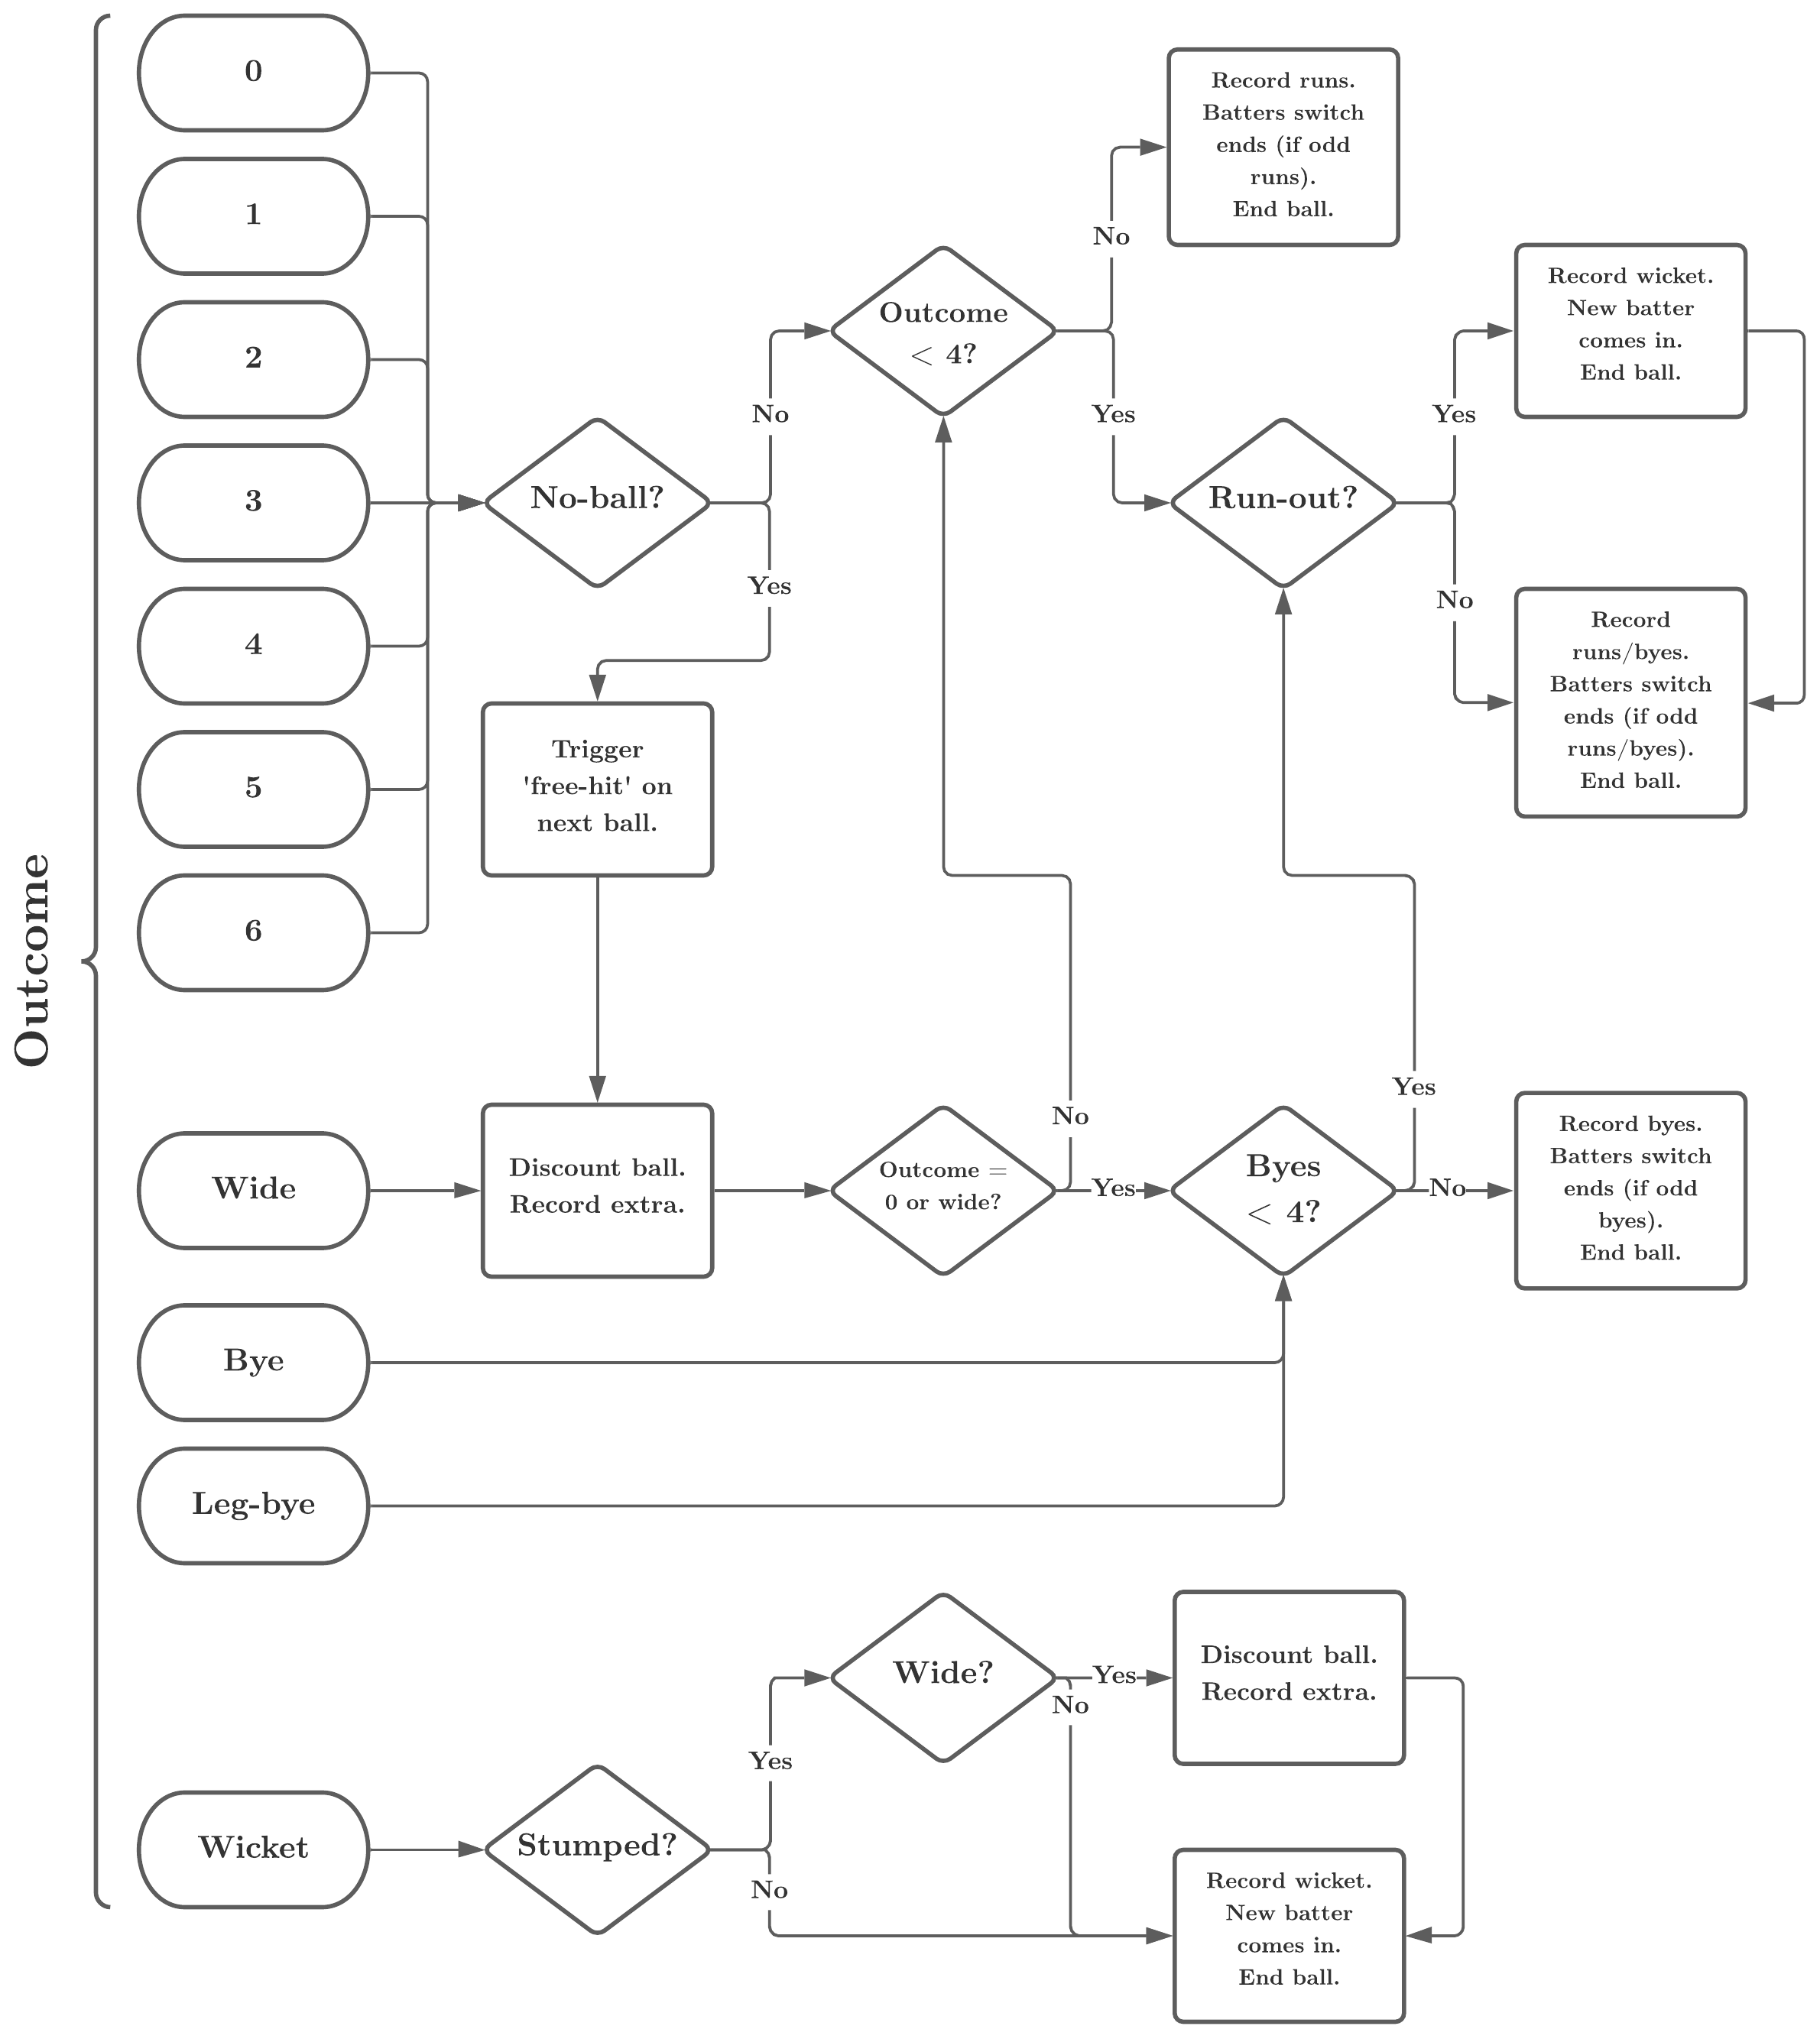
\includegraphics[width=1\columnwidth]{images/cricket flowchart (2).png}
    \caption{Flowchart showing the decision making process of the simulator during the course of a ball.}
    \label{fig: flowchart}
\end{figure}

\subsection{Simulating a Match}

Now we have a framework for how to simulate a ball, we can extend this to running through the whole match. 

\subsubsection{Pre-Match Setup}

This process begins by collecting some general information about the game which is needed for the simulator. This information includes the venue of the match, the team names of each side, and the lineups of each team. 

Team lineups are presented in the order of the batting lineup. Handy for us, since this is one less variable to estimate. However, the team lineups don't give any suggestion into the likely bowlers or order of their deployment within an innings. So this is something that we need to think about here. First I consider how many overs each player might bowl. This is inferred manually, and almost entirely based on each player's average number of overs bowled, per appearance. The number of overs each player bowls is also fixed across all simulations of the given match. This is an okay solution, but it is a shame that I wasn't able to come up with a general purpose algorithm which could perhaps be used for simulating this also. Next time! Once we have decided the number of overs each bowler is to bowl, a function is used to get the order of bowlers for each over in the innings. This is a stochastic process and does change for each new match simulation. The order is generated as follows:

\begin{enumerate}
    \itemsep-0.25em
    \item Get lineup of team along with number of overs to bowl corresponding to each player.
    \item Get list of 20 bowler names. Each name in the list represents an over to be bowled by a player in the team lineup.
    \item Shuffle the list of 20.
    \item Check to see if this is an eligible bowling order.
    \item If not, go back to step 5.
\end{enumerate}

We define a bowling order to be eligible by the following two checks. Firstly it must alternate after each over. A single player bowling two consecutive overs is forbidden in the laws of the game. Secondly, we check that of the first four and final four overs, a minimum of six of these are bowled by the best bowlers.\footnote{Bowlers bowing their maximum allocation of four overs.} This adds an extra layer of realism to the bowling orders since the important opening and closing overs tend to be the domain of the most potent bowlers.

\subsubsection{Toss}

Now we decide which team bats first in the match. In doing this we naively assume that both team's preference for batting first vs second is equal. So a simple 50:50 virtual coin toss is all that's required here.

\subsubsection{Initialising Variables}

To prepare for the start of the match we need to initialise some variables which tell the model the state of the game before each ball is simulated. Recall that these variables are altered at the end of each ball, but we need to set them up here prior to the first ball of each innings. Variables include a logical `is first innings', first innings score, batter, non-striker, next batter to enter, bowler, next bowler to bowl, current runs, wickets remaining, balls remaining, over number, ball number in the over, and the `is free hit' logical variable.

\subsubsection{Innings}

To simulate an innings we simulate an over twenty times, which itself is a repetition of the delivery simulation six times. Between deliveries, we check to see if the wickets remaining reach zero, or if the target score is reached. This signals the end of the innings/match. At the end of each over, the batters switch ends, counter variables are updated and the bowler changes.

\subsubsection{Output}

The results of a simulated match are collected in three tables. The first shows the events of each ball in every simulated match, where each row represents a ball. The second table aggregates all of these simulations and gives the results of each simulated match, where each row represents a match. The final table aggregates results from each of the matches and returns a probability of various events occurring.

Find all of the code for these processes (and the rest of the project) in the Github repository, described in \cref{appendix: code}

\section{Model Building}
\label{sec: models}

\subsection{Main Model}

The main model, used in the simulation to generate the initial outcome of a delivery, is a multi-layer perceptron. The model takes in 67 one-hot encoded variables to the input layer, which are passed through a dense hidden layer of 25 neurons, to an output layer of 11 neurons. The output layer applies the softmax activation function to each of the 11 possible outcomes, resulting in a probability estimation of each possible outcome where all 11 of these sum to 1. These are the probabilities that the simulator subsequently samples from.

\subsubsection{Input Variables}

When considering the game-state variables, I wanted to give the model a little more information than the raw numbers themselves when deducing what the relationship might be between some of these. I know from my experience watching a lot of cricket the effect that different game-states might have on the outcome of certain deliveries. For example, when the team batting first find themselves in the fortunate position of having many wickets remaining with only a couple of overs, say, remaining in their innings, they can take great risk, increasing the probability of both a boundary being scored as well a wicket falling.

We therefore include a variable derived from balls remaining and wickets remaining which I term `aggression'. This variable is simply wickets remaining divided by balls remaining and maxes out at 1. A second variable that I create from modifying the usual statistics is the required run rate. This is applicable only in the second innings and is the number of runs required to win divided again by the number of balls remaining in the innings. In games where the team batting first wins very comfortably, this number can get quickly get ridiculous. We therefore again attach a maximum value to this one of 6, since this is the highest it can possibly get before the game becomes all but theoretically out of reach for the chasing side.

When considering the batter and bowler statistics and how these should be input, I had two main concerns to address. For players with very few appearances in the data, their statistics for bowling/batting were often quite strange looking, as we might expect. We also need to think about how when it comes to testing the simulator on new games, with players that we have no data for, how we could include some other variable which could imply their ability and make an educated guess as to their possible performance.

Considering the first problem: for players with limited data, I simply removed them from the tables containing batter and bowler statistics. The restriction that I applied here was that each batter needed to have faced more than 20 deliveries, and each bowler needed to have bowled more than 3 overs in their IPL career. These choices were admittedly arbitrary, but this seemed to do the job of removing the noisy data. The secondary benefit to doing this, was that it exposed the model to the possibility of encountering new players for whom we may have no prior data for. In these instances, we should try to use some other variable that is available to us as a proxy for their possible skill and likely performance. For batters, I used the position of the batter in the batting line-up.\footnote{Batters higher up the order are generally superior to those further down.} For bowlers, I used the number of overs that the bowler is due to bowl in the innings.\footnote{In the training data I consider the average number of overs that the particular bowler bowls per innings, rounded to the nearest whole number. This is because the second innings is often concluded early meaning that not every bowler bowls their full allocation. In addition, games are occasionally curtailed due to weather, so using the actual number of overs bowled in these instances would also not be correct. I thought that average overs per appearance was therefore the best compromise, especially given that this metric was the one that I paid closest attention to in deciding the number of overs that each bowler is to bowl for each match in the 2021 season.}

So, the final list of 28 variables input to the model is as follows:
\begin{itemize}
    \itemsep-0.25em
    \renewcommand\labelitemi{-}
    \item Venue
    \item Is first innings? (logical)
    \item Is powerplay? (logical)
    \item Home advantage\footnote{Due to the circumstances of the 2021 IPL season being played during the pandemic, very few venues were used. This resulted in no team ever playing in their `home' ground. As such this variable remains set to 0 when running the simulations on the 2021 games.} - batting team (logical)
    \item Is free-hit? (logical)
    \item Aggression
    \item Required run-rate (set to 0 if `is first innings' is true.
    \item Batter position in the lineup.
    \item Batter missing from data? (logical)
    \item Batter's 0s, 1s, 2s, 4s, 6s, byes, legbyes, wickets per ball.\footnote{Set to 0 if batter data is missing.}
    \item Bowler's number of overs in the innings.
    \item Is spin bowler? (logical)
    \item Bowler missing from data? (logical)
    \item Bowler's 0s, 1s, 2s, 4s, 6s, byes, wides conceded and wickets taken per ball.\footnote{Also set to 0 if the bowler data is missing.}
\end{itemize}

These variables are fed to the model in a one-hot encoded format. This is because these types of models must have entirely numeric data fed to them. The way to solve this when working with categorical variables is to create a column for each possible category (venue, say) and use a binary 1 in the column of the venue of the particular match and 0s in all the remaining venue columns. True/false logical variables are treated in much the same way, though integers, such as batter order, are not.

\subsubsection{Hyperparameters and Tuning the Model}

Now we have all the predictor variables, formatted correctly and ready to input to the model for training. In this training phase, we use a random 90\% of the total data. The remaining 10\% is used for validation at the end. The validation process is for us to make sure that the model is behaving as it ought to be, before we come to use it for predictions on the 2021 season. It is during this training process where the model `learns' the parameters (weights and biases) of the model resulting in optimal performance. The training process itself though, is governed by more parameters and settings, set by us. These tweak the way in which the model goes about it's learning process and can have a sizeable impact on overall model performance. I chose the hyperparameters of this model, mostly through an iterative trial and error process. These decisions are outlined below.

We choose the number of hidden layers to be 1 layer of 25 nodes, with the ReLU (rectified linear unit) activation function applied to each node. I wanted to keep the model fairly simple, given my lack of experience with these methods. I initially had the number of nodes in the hidden layer set to 40 - this being the average of the number of input and output nodes which seemed a reasonable starting point. Changing this down quite a long way to 16 resulted in a slightly worse model performance (in terms of the categorical cross-entropy loss function). I subsequently tried a number somewhere in the middle and happened on a bit of a sweet-spot at 25 nodes in the hidden layer. I tried increasing the number of layers to 2 layers of 25 nodes, though this had little effect. In preference of simplicity, I retained my initial choice of one hidden layer.

The loss function that we use when evaluating the model and any changes to the hyperparameters, is the categorical cross-entropy function. This is often used in models of multi-class classification (such as this one) and it essentially measures the accuracy of the output distribution. \cite{noauthor_categorical_nodate} Other additions we make to the model are adding batch normalization and dropout regularization to the hidden layer of the network. The dropout rate (which we set here to 0.2) is where nodes in the hidden layer are randomly powered off (with probability 0.2) during the training of the model. This has the effect of reducing the network's dependence on certain nodes, forcing the network into learning a more balanced representation of the data and thus reducing over-fitting. \cite{ghatak_deep_2019} Batch normalization is another modification to the hidden layer. This normalizes the inputs to the hidden layer which makes the network faster and more stable. \cite{ioffe_batch_2015}

The model `learns' in a similar kind of trial and error way to us in the way we tweak the hyperparameters. It first looks at some rows of the data (a batch), and makes predictions for the distribution of possible outcomes. Then it tweaks those parameters used to make the prior prediction once it sees the actual outcomes that resulted from those prior sets of inputs. The loss function computes a kind of error score, quantifying the distance between the model's output and the real-life outcome. This tells the model how good or bad it's predictions were, at which point it then it goes back and alters the weights and biases of the network in such as way as to reduce the output of this loss function. It then repeats this process until the loss function reaches a local minimum. An optimizer algorithm is responsible for this process of re-tuning the weights and biases between each batch of data that the model `sees'. There are many choices available to us here - we use the Adam (adaptive moment estimation) optimizer. This function takes in another tunable parameter - the learning rate. This is a measure of how severe the changes to the model parameters are by the optimization algorithm. We set the learning rate initially to 0.0001, down from the algorithm's default value of 0.001 since the learning curve was bouncing around too much using the default learning rate value. We then ask the learning rate to reduce when the learning curve reaches a plateau, enabling finer and finer adjustments to be made to the model parameters.

The final hyperparameters we set are the maximum number of epochs that the model trains for. It is the maximum since another setting we use, tells the model to stop training when the loss function reaches its local minimum. We use 300 - a recommended setting from Ghatak's hugely helpful \textit{Deep Learning with R} \cite{ghatak_deep_2019}. This is the number of times that the model sees the entire training dataset. The batch size I set to 50 - the number of rows of the training data it looks at before altering the parameters in accordance with the Adam gradient descent function. Lastly we use a validation split of 0.1. As the model trains it tests it's current parameters on an unseen portion of the dataset (the validation set), giving us a validation loss score, as well as a training loss score.

\subsubsection{Testing the Model}

The final part of the process of developing the main model is testing it on the remaining 10\% of the data, that we set aside before training. First we take a look at the number of each outcome in the testing data, and compare this to the model's expected number of occurrences for each outcome across that same data. Given that the model gives us probabilities for each outcome, we infer its expected number for each of these by simply summing up each probability for all rows of the data.

Looking at \cref{table: main model1}, we can see that the model performs well for predicting frequencies across all categories. We judge this on the $p$ column. This $p$-value measures the probability of seeing at least the observed absolute deviation from the model's expected numbers of each outcome, under the assumption of the Poisson distribution (where $\lambda$ is the model's expected number of observations). Given all the $p$-values are above the 0.05 significance level, we can say that none of the observed number of outcomes differ significantly from the model's expectations, which is a good sign!

\begin{table}[ht]
\centering
\begin{tabular} {c c c c} \toprule
    {Outcome} & {Number Predicted} & {Number in Test Data} & {$p$} \\ \midrule
     0 & 5932.47 & 5995 & 0.413 \\
     1 & 7189.05 & 7212 & 0.781 \\
     2 & 1270.05 & 1203 & 0.060 \\
     3 & 61.64 & 67 & 0.449 \\
     4 & 2181.01 & 2181 & 0.989 \\
     5 & 6.00 & 4 & 0.570 \\
     6 & 895.26 & 870 & 0.401 \\ \midrule
     Bye & 51.88 & 41 & 0.142 \\
     Leg-bye & 317.83 & 324 & 0.702 \\
     Wicket & 864.83 & 861 & 0.914 \\
     Wide & 575.97 & 588 & 0.598 \\ \bottomrule
\end{tabular}
\caption{Performance of the main model on unseen test data.}
\label{table: main model1}
\end{table}

Most important to us in this experiment, however, is accurately predicting the total number of runs and wickets across a large sample. We can examine this in \cref{table: main model2}, where the predicted total runs is calculated by multiplying the expected number of 0s, 1s, 2s...6s from the previous table by 0, 1, 2...6. This ultimately results in a $p$-value of 0.098. Notably smaller than the mean $p$-value across the runs categories in \cref{table: main model1} (0.524), it seems we're seeing the sizable impact of scores of 6 runs already. Whilst the $p$-value for total runs is small, it remains the case that the observed total number of runs, doesn't differ significantly from expectations. This remains the case for predicting wickets, where the model performs encouragingly well.

\begin{table}[h]
\vspace{0.5em}
\centering
\begin{tabular} {c c c c} \toprule
    {Outcome} & {Total Predicted} & {Total in Test Data} & {$p$} \\ \midrule
     Runs & 24039.67 & 23783 & 0.098 \\
     Wickets & 864.83 & 861 & 0.914 \\ \bottomrule
\end{tabular}
\caption{The main model's performance on the two most important categories: total runs and wickets.}
\label{table: main model2}
\end{table}

\subsection{No-Ball Model}

Recall from \cref{sec: sim} that if the outcome sampled in the main model is from 0-6 runs, the no-ball is checked for. To sample for this we build a new model that returns the probability for a no-ball, given some inputs. In building this model, I originally attempted to use similar techniques as in the main model for predicting no-ball probability. However, the predictions made by this approach were shockingly bad. (Possibly due to a combination of the rarity of the event, and therefore a lack of no-balls amongst the training data. More likely due to my own poor tuning of the model.) Then I tried a logistic regression with several inputs that I deemed suitable (outcome, bowler, game-state, venue, bowler-type, etc.) which ultimately showed that only a single variable was significant in predicting the probability of a no-ball. This variable was the `is spin' logical. As such, our model here is refreshingly simple. If the bowler is a spin bowler, we assign a probability of the no-ball to be 0.00162. Consequently if they're a pace bowler, we set the no-ball probability to be 0.00599. These numbers are derived from the rows of data which were eligible to have been called a no-ball (i.e. not an already assigned bye, leg-bye, wide, or wicket). We split them, as before, into a training and test set using the same 90:10 ratio. Probabilities for each category are calculated as the frequentist probability of a no-ball occurring, given each bowler-type across the training data. Results of this approach on the testing set are given in the table below.

\begin{table}[h]
\vspace{0.5em}
\centering
\begin{tabular} {c c c} \toprule
    {No-Balls Predicted} & {No-Balls in Test Data} & {$p$} \\ \midrule
     77.20 & 70 & 0.451 \\ \bottomrule
\end{tabular}
\caption{Performance of the no-ball model on unseen test data.}
\label{table: noball}
\end{table}

\subsection{Byes Model}

When the simulator reaches the point in a ball simulation where the number of byes are required, it inputs to the byes model, which returns a probability distribution of possible outcomes from 0-5 byes. This is the second and final multi-class classification model after the outcome model, and is also one of the neural network variety. It uses a new variable, number of byes, as it's response. This is a number from 0-5, and represents only the number of byes scored on a given ball. So if there was a no-ball or wide, the 1 penalty run for this is not included in this count.

The inputs to this model total 7. We have logical variables for first innings, powerplay, free-hit, bowler type, the numerical game-state variables of aggression and required run rate and the category of the initial outcome. I found that a more simple tuning of the hyperparameters to this model was sufficient in obtaining a good performing model. As in the main model, we prefer simplicity here. So any additions made to the model resulting in a negligible change in performance were dropped. There is no batch normalization, nor dropout regularization applied here. The number of nodes in the hidden layer is reduced to 10 which works well. We retain the Adam optimization algorithm from the main model as well as the ReLU activation function on nodes of the hidden layer.

The model is developed using a specific subset of the ball-by-ball data where byes are possible. These are balls where the outcome is either `wide', `bye', `leg-bye', or the balls where outcome is 0 \textit{and} the `is no-ball' variable is true. This data totals just shy of 10000 rows. As before, we randomly split this up into a training and test set according to a 90:10 ratio. Below we have information on the performance of the trained byes model on the test data. Again, all $p$-values are greater than 0.05, suggesting that none of the observed counts differ significantly from the model's expectations.

\begin{table}[h]
\vspace{0.5em}
\centering
\begin{tabular} {c c c c} \toprule
    {Number of Byes} & {Number Predicted} & {Number in Test Data} & {$p$} \\ \midrule
     0 & 559.72 & 541 & 0.442 \\
     1 & 331.93 & 343 & 0.522 \\
     2 & 22.56 & 27 & 0.298 \\
     3 & 2.48 & 5 & 0.081 \\
     4 & 58.82 & 60 & 0.810 \\
     5 & 0.50 & 0 & 0.792 \\ \bottomrule
\end{tabular}
\caption{Byes model's performance on predicting the number of byes }
\label{table: byes}
\end{table}

\subsection{Run-Out Model}

The next question from the simulator that needs dealing with is deciding whether a run-out occurred on a ball for which this is a possible event. As in the previous models, we develop this model only on data for which a run-out is a possible outcome. This model is a logistic regression. It is reduced down such that only variables significant in predicting the probability of a run-out are present. This results in us using two separate models to estimate this since required run-rate (a variable only applicable in the second innings of the match) is significant. The second and final significant variable is aggression. \Cref{fig: runout} shows the relationship between run-out probability and the aggression variable nicely. This kind of relationship is expected and exactly what I hoped for. I know that many more run-outs tend to occur at the end of each innings since the batters running have far less to lose at this stage of the game. It's encouraging that this model is able to capture this.

\begin{figure}[ht]
    \centering
    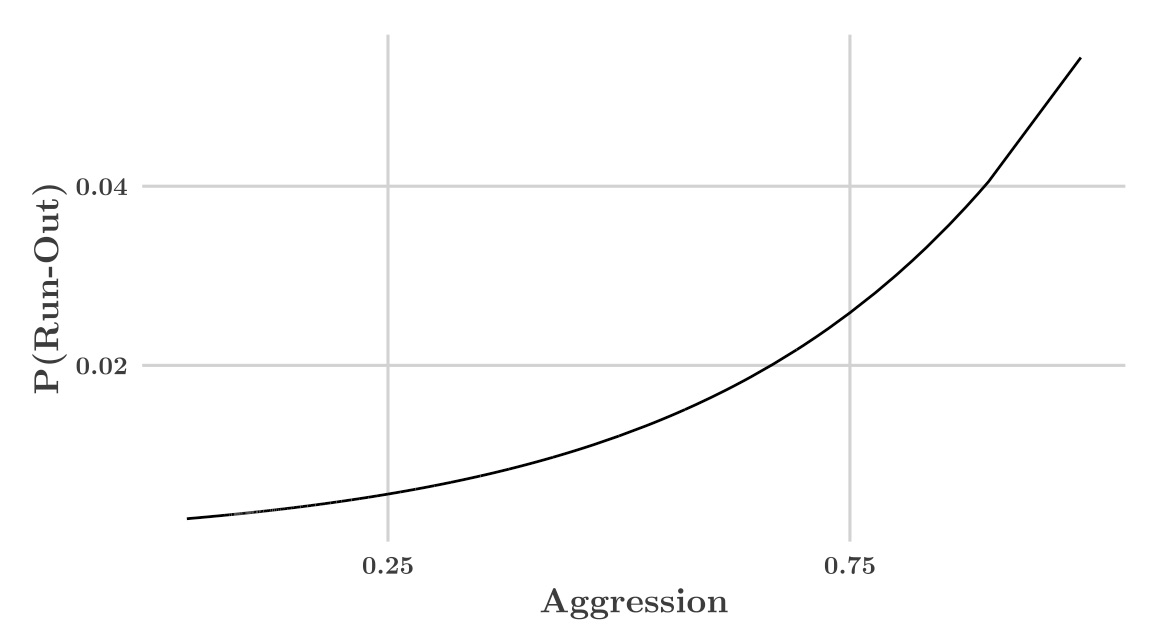
\includegraphics[width=0.75\columnwidth]{images/runoutplot2.jpeg}
    \caption{Relationship between the run-out model's predicted probability of a run-out, and the state of the innings at the time. Recall aggression is calculated as wickets remaining / balls remaining. It has a maximum value of 1.}
    \label{fig: runout}
\end{figure}

As before, we compare actual numbers of run-outs observed in the test data, against our model predictions. These $p$-values look good.

\begin{table}[ht]
\vspace{0.5em}
\centering
\begin{tabular} {c c c c} \toprule
    {Innings} & {Number Predicted} & {Number in Test Data} & {$p$} \\ \midrule
     First & 50.59 & 55 & 0.482 \\
     Second & 36.83 & 39 & 0.644 \\ \bottomrule
\end{tabular}
\caption{Run-out model's performance on predicting the number of run-outs in unseen test data.}
\label{table: runouts}
\end{table}

\newpage
\subsection{Stumped and Wide Models}

The final two areas to consider are the rare circumstances where a wicket is taken off a wide ball. This can only occur (for non-run-out wickets) if the batsman has been given out stumped. We can check for this by first evaluating the probability that a specific wicket is a stumping. If it is, we then check to see whether the delivery was a wide ball.

We first try using a logistic regression model for this. As was the case when training the no-ball model, we find that only the `is spin' logical variable is significant in predicting the probability of a stumping occurring, given the ball is a wicket. So, as before, we end up with a probability of a stumping given the bowler is a spinner (0.0986) and the probability of a stumping, given the bowler is a seamer (0.00141). 

The situation for wides on stumping balls is less clear-cut between the two types of bowlers, to the extent that no significant difference is present between the two. We use the aggregate probability figure of 0.0884 to estimate this.

These probabilities have been generated across the entire dataset (so no splitting for training/testing here). Given the lack of instances, I wanted to use as much data as I could in training these two models. It is also the case that had we split the data prior to training, we would be testing these models on a tiny test set, which wouldn't be useful.